
\documentclass[11pt,a4paper]{article}

\usepackage[utf8]{inputenc}
\usepackage[T1]{fontenc}
\usepackage{lmodern}
\usepackage[english]{babel}
\usepackage{amsmath,amsfonts,amssymb}
\usepackage{cite}
\usepackage{hyperref}
\usepackage{graphicx}
\usepackage{booktabs}
\usepackage{multirow}
\usepackage{array}
\usepackage{url}
\usepackage{xcolor}
\usepackage{enumitem}
\usepackage{float}
\usepackage{parskip}
\usepackage{microtype}
\usepackage[
  left=2.5cm,
  right=2.5cm,
  top=2.5cm,
  bottom=2.5cm,
]{geometry}

\usepackage{tikz}
\usetikzlibrary{arrows.meta, positioning, shapes.geometric, fit, backgrounds}

\hypersetup{
  pdfauthor={Ruslan Hasanov},
  pdftitle={Next-value Prediction of Sensor Data for Smart City Applications},
  pdfsubject={RCSE Research Project, Winter semester 2025/2026},
  pdfkeywords={time-series forecasting, sensor data, smart cities, LLM, zero-shot}
}

\setlength{\parindent}{0pt}
\setlength{\parskip}{5pt}

\begin{document}
\selectlanguage{english}

%%% Title %%%
\begin{titlepage}
\centering
\vspace*{2cm}
{\LARGE\bfseries Next-value Prediction of Sensor Data\\[6pt]
for Smart City Applications\par}
\vspace{1cm}
{\large Research Project Report\par}
\vspace{2cm}
\begin{tabular}{r l}
Student:    & Ruslan Hasanov \\[4pt]
Supervisor: & M.Sc.\ Timo R\"ath \\[4pt]
Chair:      & Prof.\ Patrick M\"ader \\[4pt]
Department: & DBIS, TU Ilmenau \\[4pt]
Semester:   & Winter 2025/2026 \\[4pt]
Date:       & \today \\
\end{tabular}
\vspace{1.5cm}
\begin{tabular}{l p{0.75\textwidth}}
\textbf{Keywords:} &
Time-series forecasting, Smart Cities, LLM, Zero-shot learning, Sensor data \\
\end{tabular}
\end{titlepage}


%%%%%%%%%% Abstract %%%%%%%%%%
\begin{abstract}
Smart cities have massive amounts of sensor data collected by sensors, which can be used by city managers and engineers to plan resources. We present a prototype Next Value Prediction Service (NVP-S) to predict future sensor readings from the SensBee IoT Platform using Large Language Models (LMMs) in a Zero-Shot Setting, that is, without training any model on the target sensor data.
In our NVP-S System, we first fetch a history of previous readings for each sensor. Then we normalize and serialize each reading into a string of comma-separated values, and then we prompt the LLM to continue the sequence of previous readings and filter out any output it produces that is not valid. Finally, we return an array of predicted values as well as their respective timestamps.
We compared four different models to evaluate performance: Groq Llama-3.3-70B (API), GPT-3.5-turbo-instruct (API), Llama-2-7B (Local), and Mistral-7B-v0.1 (Local). We ran each model against two real-world sensors provided by SensBee (Temperature, Visitor Count) for a total of eight different parameter configurations with three repeat runs per configuration (192 total benchmark tests), and over one thousand LLM Inference Calls. Mistral-7B-v0.1 produced the best single run results for Temperature (MAE = 0.72°C, 35.6\% better than Naive Baseline) while Llama-2-7B had the highest average results (MAE = 1.35°C). GPT-3.5-turbo-instruct failed (0\% in band accuracy) while the Instruction Tuned version of Groq Llama-3.3-70B still produced usable predictions (MAE = 1.60°C). None of the models captured the day/night pattern in visitor counts in zero-shot conditions. The ablation study confirmed three design rules: normalize input values, omit statistical context from prompts, and prefer base or lightly-tuned models over aggressively aligned variants.
\end{abstract}


%%%%%%%%%% 1. Introduction %%%%%%%%%%
\section {Introduction}
Smart cities deploy a variety of sensors across their public infrastructure, such as weather stations, turnstiles, utility meters, and traffic counters. Platforms such as SensBee collect the data generated by these sensors and provide that data in Grafana dashboards for use by operators and the public. A simple prediction of what will occur in the next couple of hours will allow operators to better staff their organizations and prepare for anticipated changes before those changes actually occur.

A practical example of this type of technology is Google’s Popular Times feature~\cite{googlepopulartimes}. This feature provides users with a graphical representation of when businesses are likely to be visited based on crowdsourced location data. An equivalent capability for smart city sensor streams will provide dashboard users with a view into what will happen going forward rather than simply a historical view of what has happened in the past. Traditional forecasting techniques such as ARIMA~\cite{taslim2024arima}, LSTM~\cite{wei2019autoencoder}, and Informer~\cite{zhou2021informer} have all been shown to generate high-quality predictions. However, each of these traditional techniques requires training on the target domain prior to generating predictions. As such, creating and maintaining multiple training pipelines for each sensor stream used on a platform such as SensBee is highly impractical.

However, Large Language Models (LLMs) provide an alternative approach to forecasting. The ability of LLMs to learn how to continue patterns learned during pre-training on large text corpora has made them capable of producing high-quality forecasts given a serialized sequence of numbers. Moreover, because the same pre-trained model can be used for forecasting temperature, visitor counts, or any other numeric sensor, the need for fine-tuning is eliminated~\cite{gruver2023llmtime}.

The purpose of this report is to describe the design and evaluation of a prototype NVP service that is integrated with the SensBee platform. The NVP service exposes a REST API, where a client sends a sensor ID, a column name, and a forecast horizon. The service then uses the provided information to retrieve recent history, run an LLM, and return a set of predicted values along with the corresponding timestamps.

\textbf{Scope Clarification.}
As part of the original research proposal, there were plans to evaluate five different models relative to one another: ARIMA, LSTM, Informer, LLMTime, and Time-LLM. After evaluating the complexity of implementing each of the five models and considering the constraints imposed by the project timeline, the scope was narrowed to include only zero-shot LLM forecasting applied to real-time data from SensBee sensors. The remaining three models are referenced in the related work section but were not evaluated as part of the project.

\textbf{Three research questions guide this work.} 
There are three research questions that are being asked within the context of this work:
\begin{enumerate}[leftmargin=*]
\item What effect do parameter configurations (normalization, prompt context, sampling temperature, sample count) have on the accuracy of the produced forecasts? 
\item Does the performance of a local 7\,B model differ from that of a cloud-hosted 70\,B API model? 
\item Is an LLM able to detect the binary day/night pattern in visitor counts (e.g., the number of visitors is significantly higher at night than during the daytime) without having access to explicit domain knowledge?
\end{enumerate}


%%%%%%%%%% 2. Related Work %%%%%%%%%%
\section{Related Work}

\begin{itemize}[leftmargin=*,topsep=0pt,itemsep=-1ex,partopsep=1ex]

\item \textbf{Statistical and deep learning models.}
ARIMA~\cite{taslim2024arima} has been developed based on linear temporal dependencies and provides accurate forecasts when the data is stationary.
Seasonal versions (SARIMA)~\cite{li2022hybrid} have been developed to account for periodicities in the data.
While these models are fast to train and relatively easy to understand, ARIMA/SARIMA are limited in their ability to capture sharp changes or nonlinear seasonal patterns.
LSTM networks~\cite{wei2019autoencoder} use gated memory cells to learn long-range dependencies and provide powerful means to model nonlinear relationships.
The Informer~\cite{zhou2021informer} extends the Transformer architecture with sparse attention to allow it to process long sequences.
Both LSTM networks and Informer are based on large amounts of labelled data and require significant computational resources (GPUs).
The necessity to maintain individual training pipelines for each sensor type requires significant development efforts.

\item \textbf{Zero-Shot Forecasting with Pre-Trained Language Models (LLMs).}
Gruver et al.~\cite{gruver2023llmtime} (LLMTime, NeurIPS 2023) used pre-trained LLMs such as GPT-3 and LLaMA-2 to demonstrate how to perform zero-shot time-series forecasting using LLMs:
(1) Normalize all inputs to a common scale,
(2) Convert the normalized inputs into a single comma-separated string,
(3) Use the string as input to an LLM and ask it to continue the string.
They determined that normalizing the input data was crucial and that including additional text prompts to the input would generally decrease performance.
Furthermore, Gruver et al. observed that instruction-tuned and chat-aligned models tend to be less effective than base models at performing numeric continuation tasks due to the fact that the training data used to fine-tune models for alignment via reinforcement learning from human feedback (RLHF) tends to emphasize explaining rather than continuing sequences of digits.

Jin et al.~\cite{jin2024timellm} (Time-LLM, ICLR 2024) froze the pre-trained LLM backbone and introduced a new trainable reprogramming layer that mapped the time series patch into a set of learned text prototype embeddings.
Compared to LLMTime, Time-LLM achieved better performance, however, the reprogramming layer had to be trained first.
One of the techniques presented by Jin et al. called Prompt-as-Prefix (i.e., prepend statistical context such as min, max, median, trend to the input), inspired one of the eight different configurations evaluated in this research.

\item \textbf{LLMs for Urban Sensor Data.}
Li et al.~\cite{li2024urbangpt} (UrbanGPT, KDD 2024) demonstrated that LLMs can be applied to urban datasets for zero-shot spatio-temporal forecasting.
Thus, Li et al.'s work demonstrates that LLMs can generalize between different domains without being retrained, which supports the application of the LLMTime-style method to smart city applications.

\end{itemize}


%%%%%%%%%% 3. System Design %%%%%%%%%%
\section{System Design}

\begin{itemize}[leftmargin=*]

\item \textbf{Architecture.}
FastAPI is used as a microservice for the NVP service and will run in its own Docker container with SensBee.
Each service can be scaled independently because it is isolated in its own containers.
The End-to-End Data Flow for a Single Forecast Request is shown in Figure~\ref{fig:pipeline}.

\item \textbf{Forecasting pipeline.}
The pipeline has six stages:
\begin{enumerate}[leftmargin=2em]
  \item \textit{Fetch history.} SensBee client sends a request with parameters \texttt{from\_time}, \texttt{to\_time}, and \texttt{time\_grouping}. Event-based sensors (e.g., visitor counts) use Max aggregation function to find peak count within each interval.
  \item \textit{Resample.} 
  History is loaded into a pandas series and resampled onto a uniform 15-minute grid. Regular sensors use forward-fill (\texttt{ffill}). Event-based sensors use forward-fill for gaps less than 2 hours (no activity during a session) and zero-fill for longer gaps (facility closed).
  \item \textit{Normalize.} The LLMTime Quantile Scaler~\cite{gruver2023llmtime} shifts the minimum down by $\beta = 0.3$ times the data range and scales so that the $\alpha = 0.95$ quantile equals ~1.0. This makes the LLM see the \emph{shape} of the data, not the magnitude or unit.
  \item \textit{Serialize.} Each normalized value is rounded to 3 decimal places and joined into a comma-separated string. LLaMA and mistral tokenize each character individually. GPT-based models need spaces between digits to prevent byte-pair encoding from merging tokens unpredictably~\cite{gruver2023llmtime}.
  \item \textit{Prompt the LLM.} 
  The system message is minimal: “You continue numerical sequences. Output only numbers separated by commas. No explanations, no text, just the numbers.”. This follows the LLMTime finding that prompts hurt performance for pure sequence continuation. The system generates $n = 5$ independent forecasts, each with sampling temperature~0.9.
  \item \textit{Parse, filter, aggregate, and denormalize.} A regex-based deserializer extracts numbers from each response. Four filters discard invalid forecasts: (a) out-of-bounds values, (b) constant or near-constant output ($\le 2$ unique values), (c) flat output (std $< 0.001$), and (d) perfectly linear trends (second derivative $< 0.005$). The median of the remaining forecasts produces the final prediction. The scaling inverse transform maps forecast values back to the original sensor units. If all forecasts are filtered, the system falls back to the last observed value (naive baseline).
\end{enumerate}

\item \textbf{REST API and caching.}
The API accepts \texttt{sensor\_id}, \texttt{column}, \texttt{horizon\_hours} (6—168), \texttt{history\_days} (1—14), \texttt{provider} (Groq, Mistral, OpenAI, or Local), and optional \texttt{model}, \texttt{num\_forecasts}, and \texttt{temperature} parameters. The service stores the most recent result for each sensor-ID + column pair in an in-memory dictionary. Repeated requests with the same key return the cached results instead of running inference again. In a production environment, a Redis cache with a TTL (e.G. 6 hours) can replace the in-memory dictionary and persist results across service restart.

\item \textbf{HPC cluster for local inference.}
Api-based models (Groq, OpenAI) take  3--9\,s per call, incur token costs, and transmit sensor data to a cloud provider.
Local inference removes all three issues.
The service was deployed on the TU Ilmenau HPC cluster with two nodes:
\begin{itemize}[leftmargin=2em,itemsep=1pt]
  \item \textit{Login node (makalu48):} Has internet access. Downloads model weights from Hugging Face into shared scratch storage.
  \item \textit{GPU node (makalu86):} 4$\times$NVIDIA A100 (40\,GB VRAM each), no internet access. Sets \texttt{HF\_HUB\_OFFLINE=1} so the transformers library loads weights from disk.
\end{itemize}
Both nodes share the \texttt{/scratch} filesystem, so the weights downloaded once on the login node are available on the GPU node without copying.
A 7\,B model requires approximately  14\,GB in \texttt{float16} and fits within one A100.

The system uses multi-GPU inference. Before each benchmark run, a VRAM check (\texttt{\_get\_usable\_gpus}) selects GPUs with at least 15\,GiB of free memory. During the experiments, three of the four A100s were available (GPU~3 was was occupied by another user with 0.2\,GiB free).
The five forecast samples were distributed across three GPUs using Python’s \texttt{ThreadPoolExecutor}, with each GPU running a separate copy of the model. Models are pre-loaded sequentially onto each GPU before parallel inference begins, which avoids file-system contention during weight loading.

\end{itemize}

%%% Figure 1: Pipeline %%%
\begin{figure}[H]
\centering
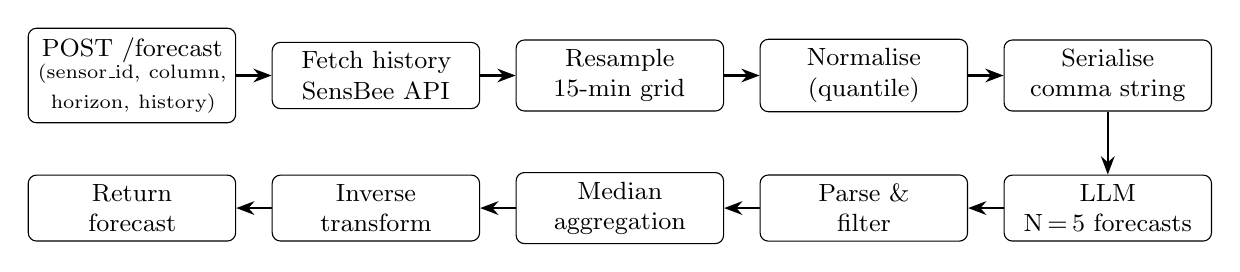
\begin{tikzpicture}[
    box/.style={rectangle, draw, rounded corners=3pt,
        minimum height=0.7cm, text width=2.4cm,
        align=center, font=\small},
    arr/.style={-{Stealth}, thick}
]
\node[box] (req) {POST /forecast\\\scriptsize(sensor\_id, column,\\horizon, history)};
\node[box, right=0.45cm of req] (fetch) {Fetch history\\SensBee API};
\node[box, right=0.45cm of fetch](prep) {Resample\\15-min grid};
\node[box, right=0.45cm of prep] (norm) {Normalise\\(quantile)};
\node[box, right=0.45cm of norm] (ser) {Serialise\\comma string};

\node[box, below=0.8cm of ser] (llm) {LLM\\N\,=\,5 forecasts};
\node[box, left=0.45cm of llm] (par) {Parse \&\\filter};
\node[box, left=0.45cm of par] (med) {Median\\aggregation};
\node[box, left=0.45cm of med] (den) {Inverse\\transform};
\node[box, left=0.45cm of den] (resp) {Return\\forecast};

\draw[arr] (req) -- (fetch);
\draw[arr] (fetch)-- (prep);
\draw[arr] (prep) -- (norm);
\draw[arr] (norm) -- (ser);
\draw[arr] (ser) -- (llm);
\draw[arr] (llm) -- (par);
\draw[arr] (par) -- (med);
\draw[arr] (med) -- (den);
\draw[arr] (den) -- (resp);
\end{tikzpicture}
\caption{End-to-end forecasting pipeline. A client request triggers history retrieval, preprocessing, LLM inference over five independent forecasts, filtering, aggregation, and inverse transformation before the result is returned.}
\label{fig:pipeline}
\end{figure}


%%%%%%%%%% 4. Data and Experimental Setup %%%%%%%%%%
\section{Data and Experimental Setup}

\subsection{Sensors}

Two of the deployed sensors by the SensBee system in Ilmenau were evaluated. These sensors are examples of the two most important sensor categories: regular-interval (or periodic) and event-based.

\begin{table}[H]
\centering
\caption{Properties of the two test sensors.}
\label{tab:datasets}
\small
\begin{tabular}{lll}
\toprule
Property         & Temperature              & Visitor count \\
\midrule
Source           & Manebach weather station & Ilmenau ice hall turnstile \\
Column           & \texttt{temperature}     & \texttt{visitors\_total} \\
Unit             & \,$^{\circ}$C            & integer count \\
Raw interval     & 15\,min (regular)        & event-based (irregular) \\
Resampled to     & 15\,min                  & 15\,min (dual-fill) \\
Points (1-day)   & 96                       & 96 \\
Observed range   & $-$12.3 to $+$8.2\,$^{\circ}$C & 0 to 125 visitors \\
\bottomrule
\end{tabular}
\end{table}

\textbf{Temperature} is a typical 15-minutes interval sensor. The temperature sensor has a strong upward trend over the observed duration due to its increasing values (from $-$12\,$^{\circ}$C to $+$8\,$^{\circ}$C), thus creating a significant macro-trend in longer input windows.

\textbf{Visitor count} is obtained from a turnstile firing a record every time someone goes into the ice-rink or out of it. Once resampled to 15 minutes, the visitor count is almost always either 0 (when the ice-rink is closed from 22:00 to 07:00) or between 20 and 125 visitors when the rink is open during weekday working hours. The rink is usually closed on Sundays. This sensor will be used to assess if an LLM is able to learn temporal rules from raw data.

\subsection{Models}

There were four models that were tested: two access methods (API and local) and two alignment types (base and instruct).

\begin{table}[H]
\centering
\caption{Models tested in the ablation study.}
\label{tab:models}
\small
\begin{tabular}{lllll}
\toprule
Model & Type & Parameters & Access & Context \\
\midrule
Groq Llama-3.3-70B   & Instruct & 70\,B   & API (Groq)   & 128\,K tokens \\
GPT-3.5-turbo-instruct & Instruct & undiscl. & API (OpenAI) & 4\,K tokens \\
Llama-2-7B           & Base     & 7\,B    & Local (HPC)  & 4\,K tokens \\
Mistral-7B-v0.1      & Base     & 7.24\,B & Local (HPC)  & 8\,K tokens \\
\bottomrule
\end{tabular}
\end{table}

In addition to instruction-tuned models: Meta’s SFT + RLHF-tuning Groq Llama-3.3-70B and OpenAI’s alignment training GPT-3.5-turbo-instruct, we have also added base models: Llama-2-7B and Mistral-7B-v0.1. According to LLMTime [Grüver et al., 2023], instruction-tuned and chat models tend to perform less well than non-chats in numerical continuation. We want to determine whether there is a dependence on the amount of alignment (i.e., if this difference is uniform).

\subsection{Ablation configurations}

Eight different configurations were used to evaluate how normalization, statistical context, sampling temperature and sample size affect the quality of forecasts made by the LLM. Each configuration is defined by its specific combination of the four variables listed above. The table below provides an overview of the variable combinations for the eight configurations used. 
In addition to the variables listed in Table~\ref{tab:configs}, every configuration has a fixed length of one day as the basis for forecasting (i.e., 96 historical data points), and uses a 24 hour forecast period (i.e., 96 forecasted points).

\begin{table}[H]
\centering
\caption{The eight ablation configurations. Check marks are included to show which features are enabled in each configuration. Every feature that is not listed in this table will be set to the baseline setting.}

\label{tab:configs}
\small
\begin{tabular}{clcccc}
\toprule
\# & Configuration & Norm. & Context & Temp. & $N$ \\
\midrule
1 & LLMTime-like (baseline) & \checkmark & $\times$ & 0.9 & 5 \\
2 & With statistical context & \checkmark & \checkmark & 0.9 & 5 \\
3 & Raw values (no normalisation) & $\times$ & $\times$ & 0.9 & 5 \\
4 & Raw values + context & $\times$ & \checkmark & 0.9 & 5 \\
5 & Low temperature & \checkmark & $\times$ & 0.7 & 5 \\
6 & High temperature & \checkmark & $\times$ & 1.0 & 5 \\
7 & 10 forecast samples & \checkmark & $\times$ & 0.9 & 10 \\
8 & 3 forecast samples & \checkmark & $\times$ & 0.9 & 3 \\
\bottomrule
\end{tabular}
\end{table}

Each configuration was run 3 times for each sensor and for each model. 
Therefore, there are 8 configurations $\times$ 2 sensors $\times$ 3~repeats $=$ 48 tests for each model and 192 tests overall for all 4~models. 
Every test will result in $N$ independent calls to the LLM for generating forecasts, resulting in more than 1{,}000 LLM inference calls in total for the entire study.

\subsection{Metrics}

\begin{table}[H]
\centering
\caption{Evaluation metrics. $f_t$ = forecast, $y_t$ = ground truth, $H$ = horizon (96 steps).}
\label{tab:metrics}
\small
\begin{tabular}{lll}
\toprule
Metric & Formula & Purpose \\
\midrule
MAE     & $\frac{1}{H}\sum|f_t - y_t|$ & Accuracy in sensor units \\[4pt]
RMSE    & $\sqrt{\frac{1}{H}\sum(f_t - y_t)^2}$ & Penalizes large spikes \\[4pt]
sMAPE   & $\frac{100}{H}\sum\frac{2|f_t-y_t|}{|f_t|+|y_t|}$ & Scale-free relative error \\[4pt]
WBA-10  & \% of steps with $|f_t - y_t| \le 0.1 \cdot \text{range}$ & Within-band success rate \\[4pt]
vs.\ Naive & $100 \cdot \frac{\text{MAE}_{\text{naive}} - \text{MAE}_{\text{model}}}{\text{MAE}_{\text{naive}}}$ & Improvement over last-value baseline \\
\bottomrule
\end{tabular}
\end{table}

The \emph{naive baseline} always uses the same value as the previous step to make predictions for all subsequent steps. For the test data, the naive baseline has an MAE of 1.115\,$^{\circ}$C for temperature and an MAE of 18.698 for visitors. A positive value for the vs. Naive metric means the model performed better than the naive baseline. Otherwise, it indicates the naive baseline was better.


%%%%%%%%%% 5. Results %%%%%%%%%%
\section{Results}

\subsection{Temperature}

Overall performance for each of the three models tested is shown in Table~\ref{tab:temp_overall}. Each model's overall performance is based on averaging the MAE of each of the 24~runs (8~different configurations $\times$ ~3~runs per configuration). The last two columns of the table show the best run for each model.

\begin{table}[H]
\centering
\caption{Temperature results---overall averages and best single run per model. Naive baseline: MAE\,=\,1.115\,$^{\circ}$C.}
\label{tab:temp_overall}
\small
\begin{tabular}{l rrrr r rr}
\toprule
 & \multicolumn{4}{c}{Average across 24 tests} & & \multicolumn{2}{c}{Best single run} \\
\cmidrule(lr){2-5} \cmidrule(lr){7-8}
Model & MAE & RMSE & WBA-10 & vs.N & & MAE & vs.N \\
\midrule
Llama-2-7B       & 1.35 & 1.61 & 22.3\% & $-$21.6\% && \textbf{0.85} & $+$23.8\% \\
Mistral-7B-v0.1  & 1.55 & 1.85 & 24.3\% & $-$39.4\% && \textbf{0.72} & $+$35.6\% \\
Groq 70B         & 1.60 & 2.00 & 20.0\% & $-$43.5\% && 0.96 & $+$14.3\% \\
GPT-3.5-instruct & 4.00 & 4.13 &  0.0\% & $-$258.9\% && 3.32 & $-$197.7\% \\
\bottomrule
\end{tabular}
\end{table}

Of these four models, \textbf{Llama-2-7B} produced the best average MAE at 1.35 \, $^{\circ}$C, with the lowest standard deviation between all models in all configurations. Additionally, Llama-2-7B produced the lowest MAE of any model on the single run level with a MAE of 0.85\,$^{\circ}$C using the ``Raw Values + Context'' configuration, which beat the naive baseline by 23.8\%.

\textbf{Mistral-7B-v0.1} produced the lowest single run MAE of any model at 0.72\,$^{\circ}$C using the ``LLMTime-like Baseline'' configuration, while beating the naive baseline by 35.6\%. However, the same configuration resulted in some of the higher outlier runs for the model as well, which increased the overall average to 1.55\,$^{\circ}$C.

\textbf{Groq Llama-3.3-70B} had an average MAE of 1.60\,$^{\circ}$C across all of its configurations. The model's best single run MAE was 0.96\,$^{\circ}$C and occurred when forecasting three samples. Inference time for this model ranged from 2 to 14 seconds per test using the cloud API.

\textbf{GPT-3.5-turbo-instruct} failed in all of the configurations tested. Regardless of whether the input was normalized or raw, whether statistical context was included in the prompt, or what temperature settings were used, the model produced nearly identical output, resulting in a MAE of about 3.3\,$^{\circ}$C for normalized inputs and a MAE of 6.0\,$^{\circ}$C for raw inputs. Therefore, the LLMTime conclusion that instruction-tuned models do not perform well for numeric sequence continuation holds true for GPT-3.5-turbo-instruct.

\subsection{Temperature ablation by configuration}

Ablation testing was performed to determine how different configurations impacted each of the three base models' ability to predict temperature sequences. The results of the ablation testing are shown in Table~\ref{tab:temp_ablation}. GPT-3.5-instruct is not included in this table since it produced identical results in all of the configurations tested.

\begin{table}[H]
\centering
\caption{Temperature MAE (\,$^{\circ}$C) per ablation configuration, averaged over 3 repeats.
Bold = lowest MAE for that model. Naive baseline = 1.115\,$^{\circ}$C.}
\label{tab:temp_ablation}
\small
\begin{tabular}{l ccc r rrr}
\toprule
 & Norm & Ctx & \multicolumn{1}{c}{Settings} & Groq 70B & Llama-2 & Mistral & Mean \\
\midrule
Baseline          & \checkmark & $\times$ & $T$=0.9, $N$=5 & 2.11 & 1.17 & 0.93 & 1.40 \\
+\,Context        & \checkmark & \checkmark & $T$=0.9, $N$=5 & 1.58 & 1.31 & 1.32 & 1.40 \\
Raw values        & $\times$ & $\times$ & $T$=0.9, $N$=5 & 2.19 & 1.39 & 1.62 & 1.73 \\
Raw + context     & $\times$ & \checkmark & $T$=0.9, $N$=5 & 1.46 & 1.07 & 2.80 & 1.78 \\
Low temp          & \checkmark & $\times$ & $T$=0.7, $N$=5 & 1.41 & 1.24 & 1.77 & 1.47 \\
High temp         & \checkmark & $\times$ & $T$=1.0, $N$=5 & 1.37 & 1.88 & \textbf{0.92} & 1.39 \\
10 samples        & \checkmark & $\times$ & $T$=0.9, $N$=10 & \textbf{1.18} & \textbf{0.98} & 1.05 & \textbf{1.07} \\
3 samples         & \checkmark & $\times$ & $T$=0.9, $N$=3 & 1.49 & 1.81 & 2.01 & 1.77 \\
\bottomrule
\end{tabular}
\end{table}

\textbf{Key findings from the ablation:}

\begin{itemize}[leftmargin=*]
\item \textbf{More forecast samples reduces variance.} (mean MAE\,=\,1.07\,$^{\circ}$C). Averaging across the three base models, there is a significant improvement in temperature prediction accuracy when using 10 samples instead of 3 samples (mean MAE: 1.07\,$^{\circ}$C vs.\ 1.77\,$^{\circ}$C).

\item \textbf{Normalizing inputs improves predictions for larger models, but not uniformly.} Normalizing inputs improved predictions for larger models (Groq 70B and Mistral-7B), but did not improve predictions for Llama-2-7B (it actually reduced them). 
  For Groq 70B, normalized configurations averaged 1.52\,$^{\circ}$C vs.\ 1.82\,$^{\circ}$C for raw configurations ($-$17\,\%).
  For Mistral-7B, normalized averaged 1.33\,$^{\circ}$C vs.\ 2.21\,$^{\circ}$C for raw ($-$40\,\%).
  For Llama-2-7B, normalized averaged 1.40\,$^{\circ}$C vs.\ 1.23\,$^{\circ}$C for raw ($+$14\,\%).  
  
\item \textbf{Adding statistical context had an inconsistent effect.}
  dding statistical context improved predictions for Groq 70B (2.11\,$\to$\,1.58) but appeared to have a slight negative effect on the local models.

\item \textbf{Sampling temperature affected models differently.}
  Lower temperatures (0.7) improved Groq 70B and Llama-2-7B, but negatively impacted Mistral-7B. Higher temperatures (1.0) improved Mistral-7B (0.92\,$^{\circ}$C, second-best config) and negatively impacted Llama-2-7B (1.88\,$^{\circ}$C).

\end{itemize}


\subsection{Visitor count}

In table~\ref{tab:vis_overall}, we show the average visitor count results over all three models in total.

\begin{table}[H]
\centering
\caption{Visitor count results---overall averages per model. Naive baseline: MAE\,=\,18.698 visitors.}
\label{tab:vis_overall}
\small
\begin{tabular}{l rrrr}
\toprule
Model & Avg MAE & Avg WBA-10 & Avg vs.N & Best MAE \\
\midrule
GPT-3.5-instruct & 18.70 & 54.2\% & $+$0.0\% & 18.69 \\
Groq 70B         & 20.82 & 52.8\% & $-$11.4\% & 18.70 \\
Llama-2-7B       & 30.67 & 48.3\% & $-$64.0\% & 18.70 \\
Mistral-7B-v0.1  & 44.02 & 48.7\% & $-$135.4\% & 18.70 \\
\bottomrule
\end{tabular}
\end{table}

None of our models have generated forecasts with better accuracy than the naive baseline for predicting visitor numbers. The best MAE for all our models is about 18.70 -- identical to that of the naive baseline. This number always occurs when \emph{all} of the forecast samples fail the quality filter and fall into the category of simply repeating the last observed value.

As you would expect, the higher averages for the local models (30.67 and 44.02) are due to occasional extremely poor performance on the part of a single unfiltered forecast sample which resulted in extreme values being reported (for example, one of the Mistral-7B runs produced an MAE of 406.8).

The 54.2\,\% WBA-10 is deceptive. Due to the inclusion of overnight hours, it is artificially inflated because at those times the ground truth and the forecast will be close to zero, each step will fall within the tolerance band regardless of whether or how well the model was able to make a prediction. During the day (10:00--20:00), the model consistently under-predicted the number of visitors.

All of our models and configurations produced normalized visitor data that were essentially constant or nearly so, as they mapped almost all visitor values (which are usually 0 during closing hours) to the scaler minimum (\( \approx -0.99 \)), and the LLM repeated this constant value. When raw-value configurations did produce some non-constant output, their corresponding forecasts were generally worse than naive.


%%%%%%%%%% 6. Discussion %%%%%%%%%%
\section{Discussion}

\begin{itemize}[leftmargin=*]

\item \textbf{Tuning of instructions and numeric continuation.}
GPT-3.5-turbo-instruct achieved a WBA-10 of 0\,\% on temperature across all 24~tests.
It generated nearly the same output for every configuration.
In early experiments using Llama-2-7B-Chat and Mistral-7B-Instruct-v0.2 (not included in the full ablation study) we observed the same behavior: the chat model produced the same output everywhere ($\sim$0.47), while the instruct model produced declining linear trends.
However, the instruction-tuned (SFT\,+\,RLHF) Groq Llama-3.3-70B---still produced usable forecasts (average MAE\,=\,1.60\,$^{\circ}$C).
There are two reasons why we see this difference: (1)~Meta’s alignment for Llama~3.3 is less strict than OpenAI’s RLHF; therefore, more of the original model’s ability to continue patterns will remain; (2)~with its 70\,B parameter count, the model has enough representational power to maintain its numeric skills after being tuned by the instructions.

The important takeaway is that instruction-tuned models do not all fail in the same way. Rather, it matters how much and what type of alignment is done.

\item \textbf{Smaller base models can be better than an instruction-tuned large base model.}
On average, both of the 7\,B base models performed better than the 70\,B instruction-tuned Groq model on average MAE for temperature (Llama-2-7B: 1.35, Mistral-7B: 1.55, Groq: 1.60).
There could be two contributing factors to this: (1)~Instruction tuning can cause the model to favor explanation over continuation and thus increase the amount of error and (2)~The 70\,B model has more representational capacity than the 7\,B models to hold more patterns. Therefore, it tends to extrapolate more strongly the dominant macro-trend in the input.
When the input includes a multi-day rising temperature trend, the larger model continues the trend instead of continuing the local daily cycle.
The 7\,B base models have less representational capacity than the 70\,B model and no alignment overhead. Therefore, they tend to continue more conservatively.

\item \textbf{Why does visitor forecasting fail?}
The visitor signal has a sharp binary structure: 0 at night, 20--125 during the day.
The model learns to continue the low constant value after normalization, where the overnight zeros dominate the sequence (approximately 40\,\% of a 1-day window).
Without normalization, the raw values range from 0 to 125, but the model still does not learn to make the sharp transitions at opening and closing times.
A domain-specific rule (e.g., "Set the forecast to 0 if time is outside 07:00-22:00") would improve the result without changing the model.

\item \textbf{Variability across runs.}
We saw variability in the results across repeated configurations of the same model (e.g., the MAE of the Mistral-7B baseline varied from 0.72 to 1.24 across the three repeats).
This variability is inherent to the sampling process of LLMs with temperature set to 0.9.
The filtering mechanism increases the variability of the results: When one of five forecasts is rejected, the median of the remaining four forecasts shifts substantially.
With ten samples, $N = 10$, we were able to reduce this effect (the mean MAE was 1.07 across the three functional models) but at the cost of doubling the inference time.

\item \textbf{Comparison to results in the LLMTime paper.}
Gruver et al.~\cite{gruver2023llmtime} reported competitive performance of LLMs compared to purpose-built models on standard benchmarks (Monash, Darts).
The smart city sensor data in our project has other challenges: The temperature data has a strong macro-trend, and the visitor data has a binary day/night structure.
These patterns are difficult for zero-shot LLMs as the models lack domain knowledge about opening hours and cannot distinguish seasonal trends from noise.

\item \textbf{Inference time.}
All API-based models (Groq, OpenAI) required 1--14\,s to complete each test.
For the HPC-cluster the 7\,B models required 20--55\,s per test on a single GPU, and roughly the same distributed across three GPUs (the model loading overhead balances the benefits of parallelism for the relatively small workload of $N = 5$).

Model-loading costs additional 6--8\,s for the first test. After that, subsequent tests use the cached model loaded into the GPU memory.
\end{itemize}


%%%%%%%%%% 7. Limitations and Conclusion %%%%%%%%%%
\section{Limitations and Conclusion}
\label{sec:limitations}

\subsection{Limitations}

\begin{itemize}[leftmargin=*]
  \item \textbf{Limited scope.} 
  The three baseline models — ARIMA, LSTM, and Informer — were originally intended as baselines. Because of the time constraints and the complexity of the implementation, only the naive last-value baseline was used as a reference model.
  
  \item \textbf{Single input window.} The systematic ablation study used only a 1-day input window (96 points). Preliminary tests with 3-day, 7-day, and 14-day windows showed that longer windows degraded performance for the larger Groq 70B model (macro-trend extrapolation). A full window-size sweep with the current code is future work.
  \item \textbf{Token budget.} A 7-day window at 15-minute resolution produces 672 values. The 14-day window (1{,}344 values) exceeds the 4{,}096-token context limit of Llama-2-7B. Reducing the time resolution to hourly would cut the token count by 4$\times$ but lose intra-hour variation.
  \item \textbf{No fine-tuning.} All models use generic pretraining knowledge. The models know nothing about SensBee sensors, the ice hall schedule, or local climate patterns. A fine-tuned or few-shot-adapted model would likely improve results for both sensor types.
  \item \textbf{Stochastic variance.} Temperature results vary across runs (e.g.\ Mistral-7B baseline MAE ranged from 0.72 to 1.24 across three repeats). The median is sensitive when samples are discarded: with $N = 5$, losing one sample shifts the median noticeably.
  \item \textbf{Visitor count quality.} Neither the 7\,B base models nor the 70\,B instruction-tuned model captured the day/night pattern. WBA-10 of 54.2\,\% overestimates accuracy because overnight zero-steps inflate the within-band count.

  \item \textbf{Single input window.} A single 1-day input window (96 points) was used in the systematic ablation study. Tests with longer input windows — 3 days, 7 days, and 14 days — showed that longer input windows decrease performance of the larger Groq 70B model (macro trend extrapolation). Therefore, a full window size sweep with the current code is a subject of future research.
  
  \item \textbf{Token budget.} A 7-day window at 15-minute resolution will create 672 values. Using a 14-day window (1344 values), which is beyond the 4096 tokens that define the context limit of Llama-2-7B. However, reducing the time resolution to hourly would reduce the number of tokens by 4 times and discard intra-hour variability.
  
  \item \textbf{No fine-tuning.} All models are trained with general pre-training knowledge. The models have no information regarding the SensBee sensors, the ice-hall schedule, or the local climate patterns. Fine-tuning or few-shot adaptation of the models would most probably lead to better results for both sensor types.

  \item \textbf{Stochastic variance.} Temperature results are different across the runs (for example, the range of MAE for Mistral-7B baseline varied from 0.72 to 1.24 across three repeats). The median is very sensitive to lost samples: if you lose one sample, the median will be changed significantly even though $N = 5$.
  
  \item \textbf{Visitor count quality.} Neither the 7\,B base models nor the 70\,B instruction-tuned model capture the day/night pattern. WBA-10 of 54.2 \% overestimates accuracy since overnight zero-steps increase the within-band count. 
  
\end{itemize}

\subsection{Conclusion}

This project has developed a zero-shot forecasting service based on LLM for smart city sensor data and tested it on two real sensors of the SensBee platform with four models and eight parameter combinations.

There are three notable results:

\begin{enumerate}[leftmargin=*]
    \item \textbf{The base 7\,B models exceed an instruction-tuned 70\,B API model in terms of temperature.}
    Llama-2-7B averaged MAE\,=\,1.35\,$^{\circ}$C and Mistral-7B-v0.1 had the best single result (MAE\,=\,0.72\,$^{\circ}$C, $+$35.6\,\% compared to naive).
    The instruction-tuned 70\,B Groq model averaged 1.60\,$^{\circ}$C.
    Smaller base models tend to produce more conservative continuations and therefore are less susceptible to macro trend extrapolation.
    
    \item \textbf{Too aggressive alignment causes loss of numeric continuation, but light tuning does not.}
    GPT-3.5-turbo-instruct scored 0 \% WBA-10 in all 24 temperature tests. Groq Llama-3.3-70B, also instruction-tuned, still generated useful predictions (avg MAE\,=\,1.60\,$^{\circ}$C). The way and the degree of alignment training determine whether numeric continuation is preserved.
    
    \item \textbf{Forecasting of the visitor count remains unresolved in the zero-shot mode.}
    None of the models have identified the binary open / closed pattern. Rules specific to the domain or fine-tuning are necessary.
\end{enumerate}
 
Three design principles supported by the ablation are:
\begin{itemize}[leftmargin=*] 
    \item Normalize input (the quantile scaler improved MAE for 2 of the 3 functional models).
    \item Exclude statistical context from prompt (it disrupts sequence continuation).
    \item Forecast with a higher number of forecast samples (N = 10 resulted in the smallest average MAE among the three functional models: 1.07\,$^{\circ}$C).
\end{itemize}

\subsection{Future work}

\begin{itemize}[leftmargin=*]
    \item Conduct a complete window-size sweep (1, 3, 7, 14~days) with the current code base.
    \item Implement ARIMA as a classical baseline for direct comparison.
    \item Incorporate a closing hours rule for visitor type sensors to handle the binary day/night pattern.
    \item Use Redis instead of an in-memory cache for production deployments.
    \item Test larger local models (for example, 13 B, 70 B) on the HPC cluster using model parallelization on the four A100 GPUs.
\end{itemize}


%%%%%%%%%% References %%%%%%%%%%
{
\small
\begingroup
\let\chapter\section
\begin{thebibliography}{10}

\bibitem{gruver2023llmtime}
N.~Gruver, M.~Finzi, S.~Qiu, and A.~G.~Wilson,
``Large language models are zero-shot time series forecasters,''
in \textit{Advances in Neural Information Processing Systems (NeurIPS)},
2023, pp.\ 19622--19635.
[Online]. Available: \url{https://arxiv.org/abs/2310.07820}

\bibitem{jin2024timellm}
M.~Jin, S.~Wang, L.~Ma, Z.~Chu, J.~Y.~Zhang, X.~Shi, P.-Y.~Chen,
Y.~Liang, Y.-F.~Li, S.~Pan, and Q.~Wen,
``Time-LLM: Time series forecasting by reprogramming large language models,''
in \textit{International Conference on Learning Representations (ICLR)},
2024.
[Online]. Available: \url{https://arxiv.org/abs/2310.01728}

\bibitem{taslim2024arima}
D.~Taslim and I.~Murwantara,
``Comparative analysis of ARIMA and LSTM for predicting fluctuating time
series data,''
\textit{Bulletin of Electrical Engineering and Informatics},
vol.\ 13, no.\ 3, pp.\ 1943--1951, 2024.
[Online]. Available: \url{https://doi.org/10.11591/eei.v13i3.6034}

\bibitem{wei2019autoencoder}
W.~Wei, H.~Wu, and H.~Ma,
``An autoencoder and LSTM-based traffic flow prediction method,''
\textit{Sensors}, vol.\ 19, no.\ 13, p.\ 2946, 2019.
[Online]. Available: \url{https://doi.org/10.3390/s19132946}

\bibitem{zhou2021informer}
H.~Zhou, S.~Zhang, J.~Peng, S.~Zhang, J.~Li, H.~Xiong, and W.~Zhang,
``Informer: Beyond efficient transformer for long sequence time-series
forecasting,''
in \textit{AAAI Conference on Artificial Intelligence},
2021, pp.\ 11106--11115.
[Online]. Available: \url{https://doi.org/10.1609/aaai.v35i12.17325}

\bibitem{li2022hybrid}
G.~Li and N.~Yang,
``A hybrid SARIMA-LSTM model for air temperature forecasting,''
\textit{Advanced Theory and Simulations}, vol.\ 6, no.\ 2, 2022.
[Online]. Available: \url{https://doi.org/10.1002/adts.202200502}

\bibitem{li2024urbangpt}
Z.~Li, L.~Xia, Y.~Xu, and C.~Huang,
``UrbanGPT: Spatio-Temporal Large Language Models,''
in \textit{ACM SIGKDD}, 2024, pp.\ 5351--5362.
[Online]. Available: \url{https://doi.org/10.1145/3637528.3671578}

\bibitem{googlepopulartimes}
Google LLC,
``Popular times, wait times, and visit duration,''
[Online]. Available:
\url{https://support.google.com/business/answer/6263531?hl=en}
(accessed Feb.\ 2026)

\end{thebibliography}
\endgroup
}

\end{document}
